\begin{figure}[h]
\centering
\includegraphics[width=\textwidth]{concept-fig}
\caption{Conceptual overview of method. For each local tree we use the dynamic
programming method of \citet{Sankoff_Rousseau_1975} to fit a minimum cost
dispersal surface to the genealogical relationships of the georeferenced sample
nodes. In this example, we use squared Euclidean distance as the cost function 
and $f_u(x,y)$ returns the smallest sum of squared dispersal distances between 
all ancestor-descendant node pairs that can be obtained when node $u$ is at 
location $(x,y)$. Using the genomic spans of local trees as weights, we then 
take a weighted average of local surfaces to assign each node a single average 
minimum cost dispersal surface. Here, node 4 appears in all three 
local trees and its final fitted surface is the weighted average of the three 
local surfaces. By contrast, nodes 3, 5, and 6 appear in a single local tree 
and their final fitted surfaces are identical to the surface in the local tree 
in which they appear. The perspective plot in the rightmost panel displays the
ancestral recombination graph encoding the local trees along with the final 
fitted surface for each node. Non-sample nodes are positioned at the minimum cost 
point on the surface (warmer colors denote higher costs). Note that we also 
estimate surfaces for sample nodes but these are omitted for clarity. 
}
\label{fig:concept-fig}
\end{figure}

\begin{figure}[h]
\centering
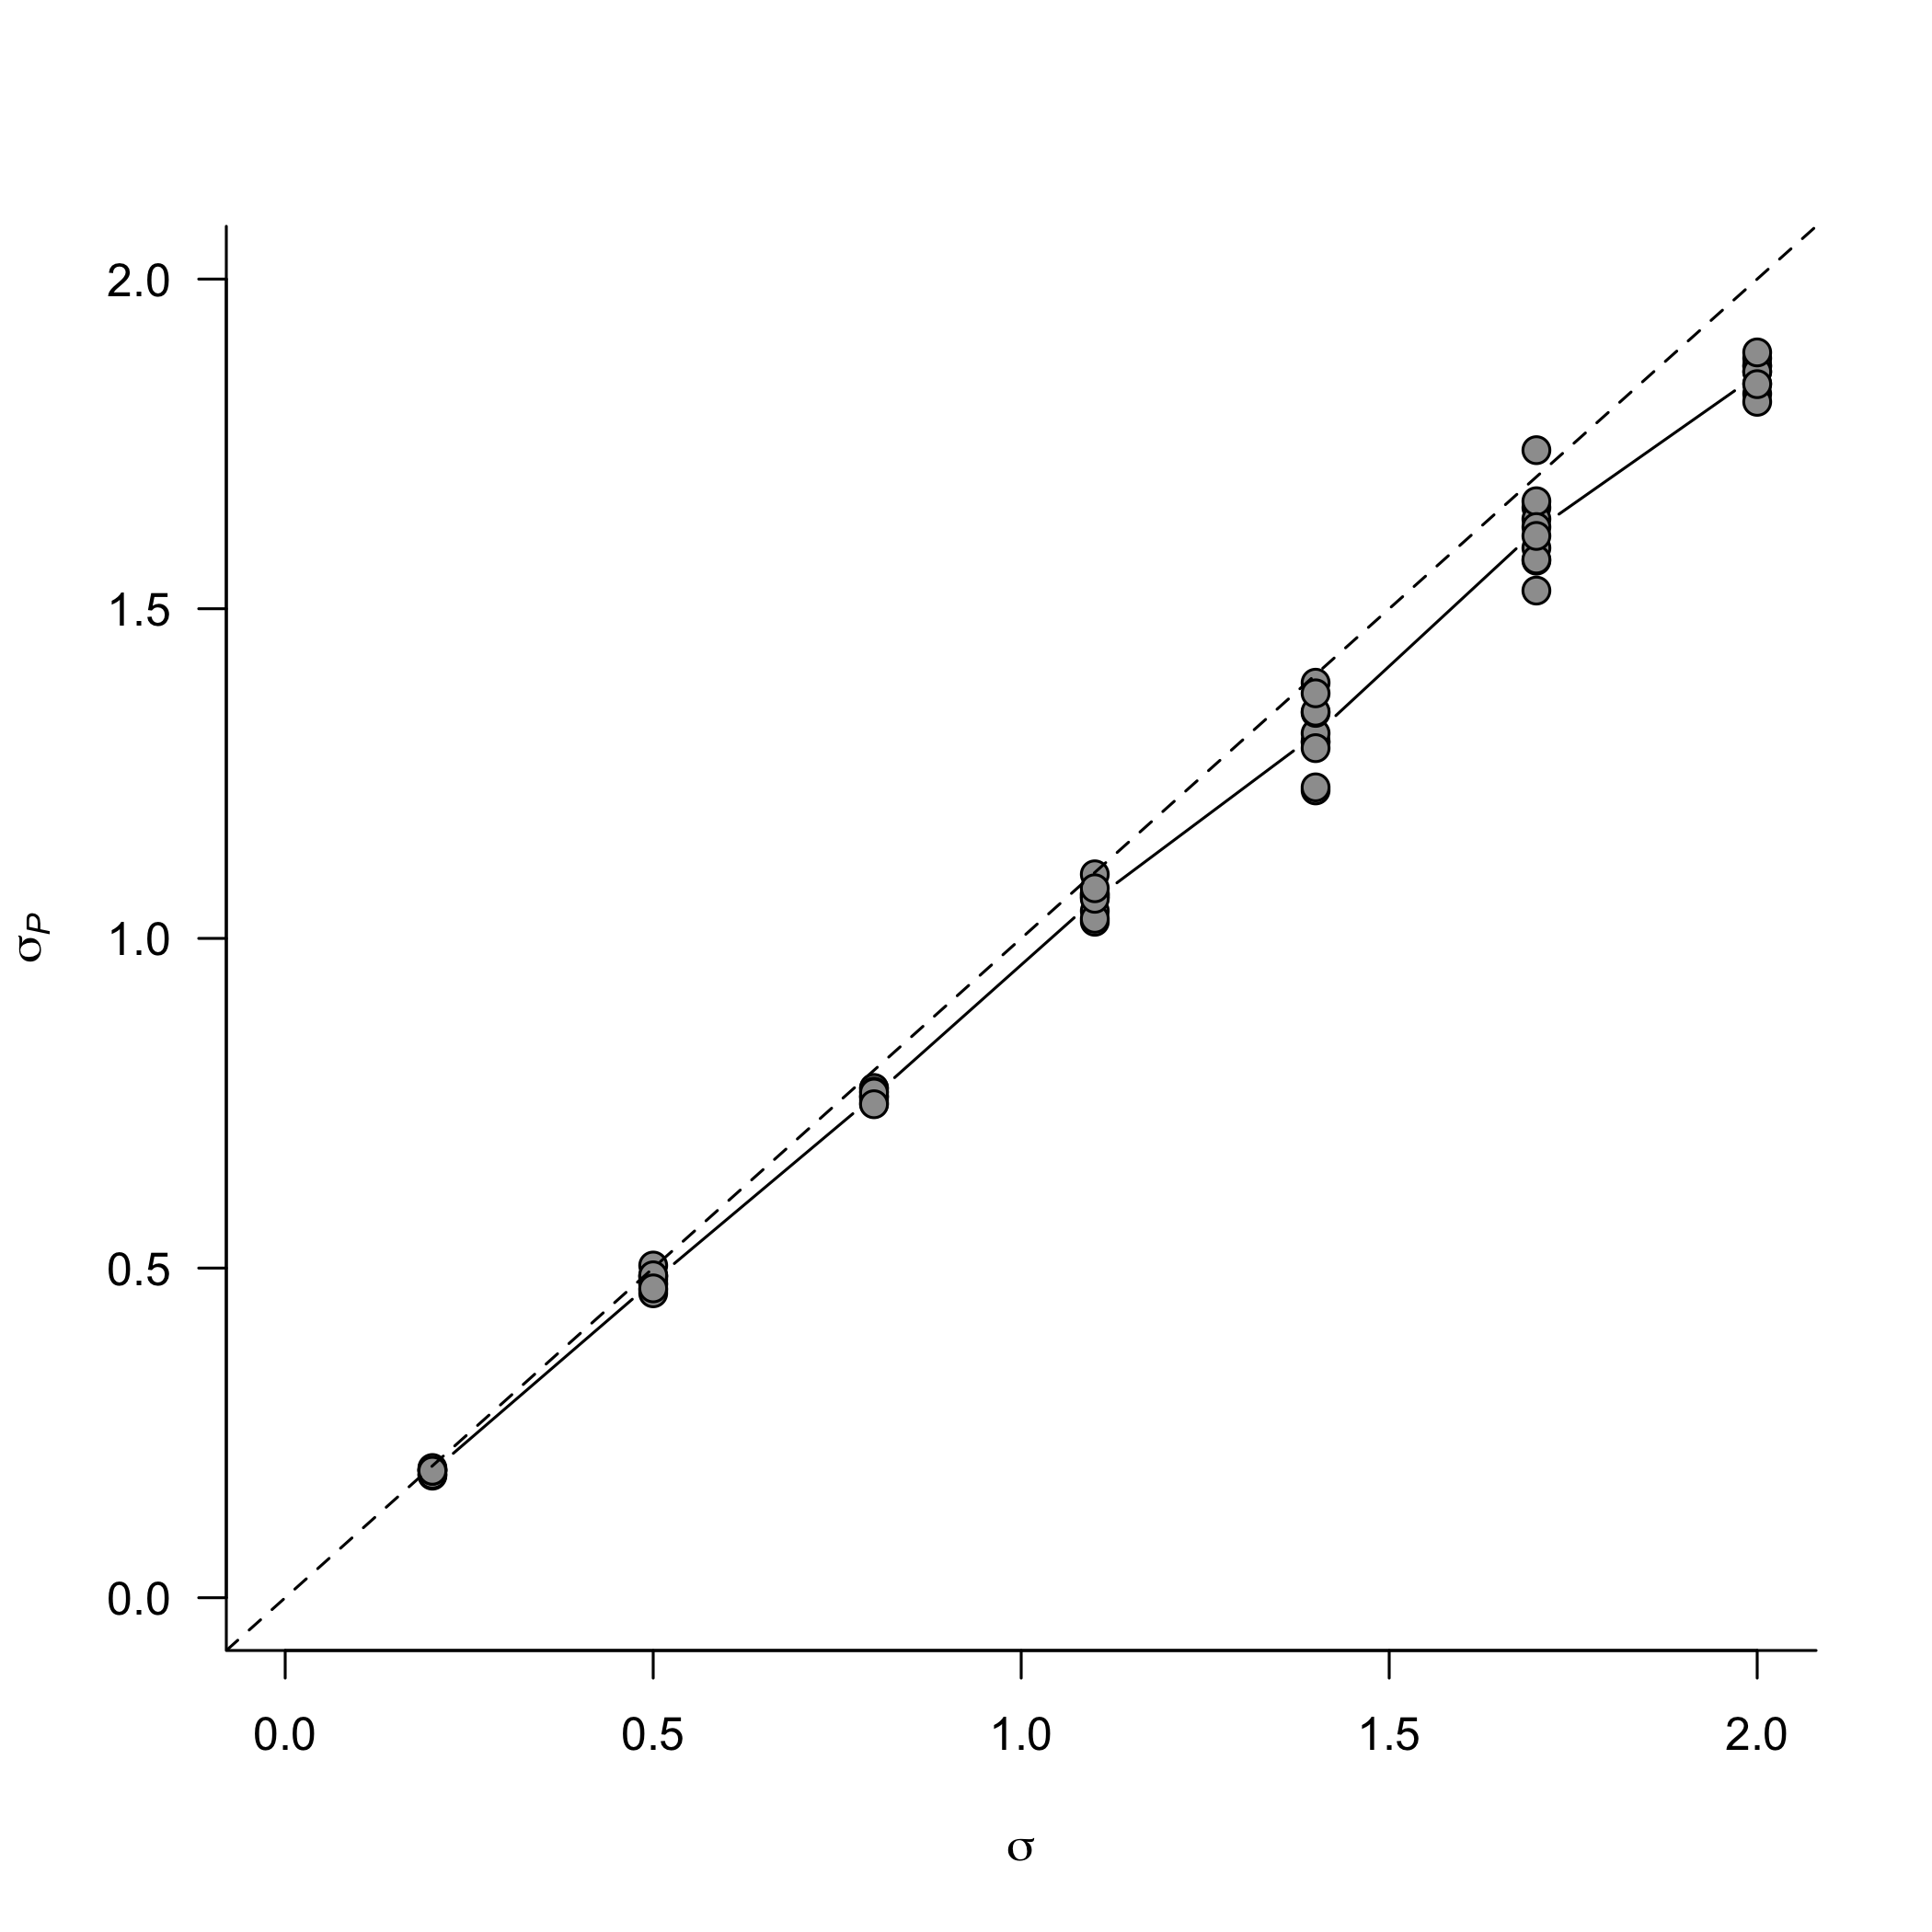
\includegraphics[width=\textwidth]{gauss-kernel-rate-estimates}
\caption{Migration rate estimates for a Gaussian dispersal kernel. Each point
represents a single simulation generated under Gaussian dispersal with effective
migration rate given on the x-axis and a parsimonious genome-wide estimate of that
rate on the y-axis. The inset line shows a 1:1 relationship.
}
\label{fig:gauss-kernel-rate-estimates}
\end{figure}

\begin{figure}[h]
\centering
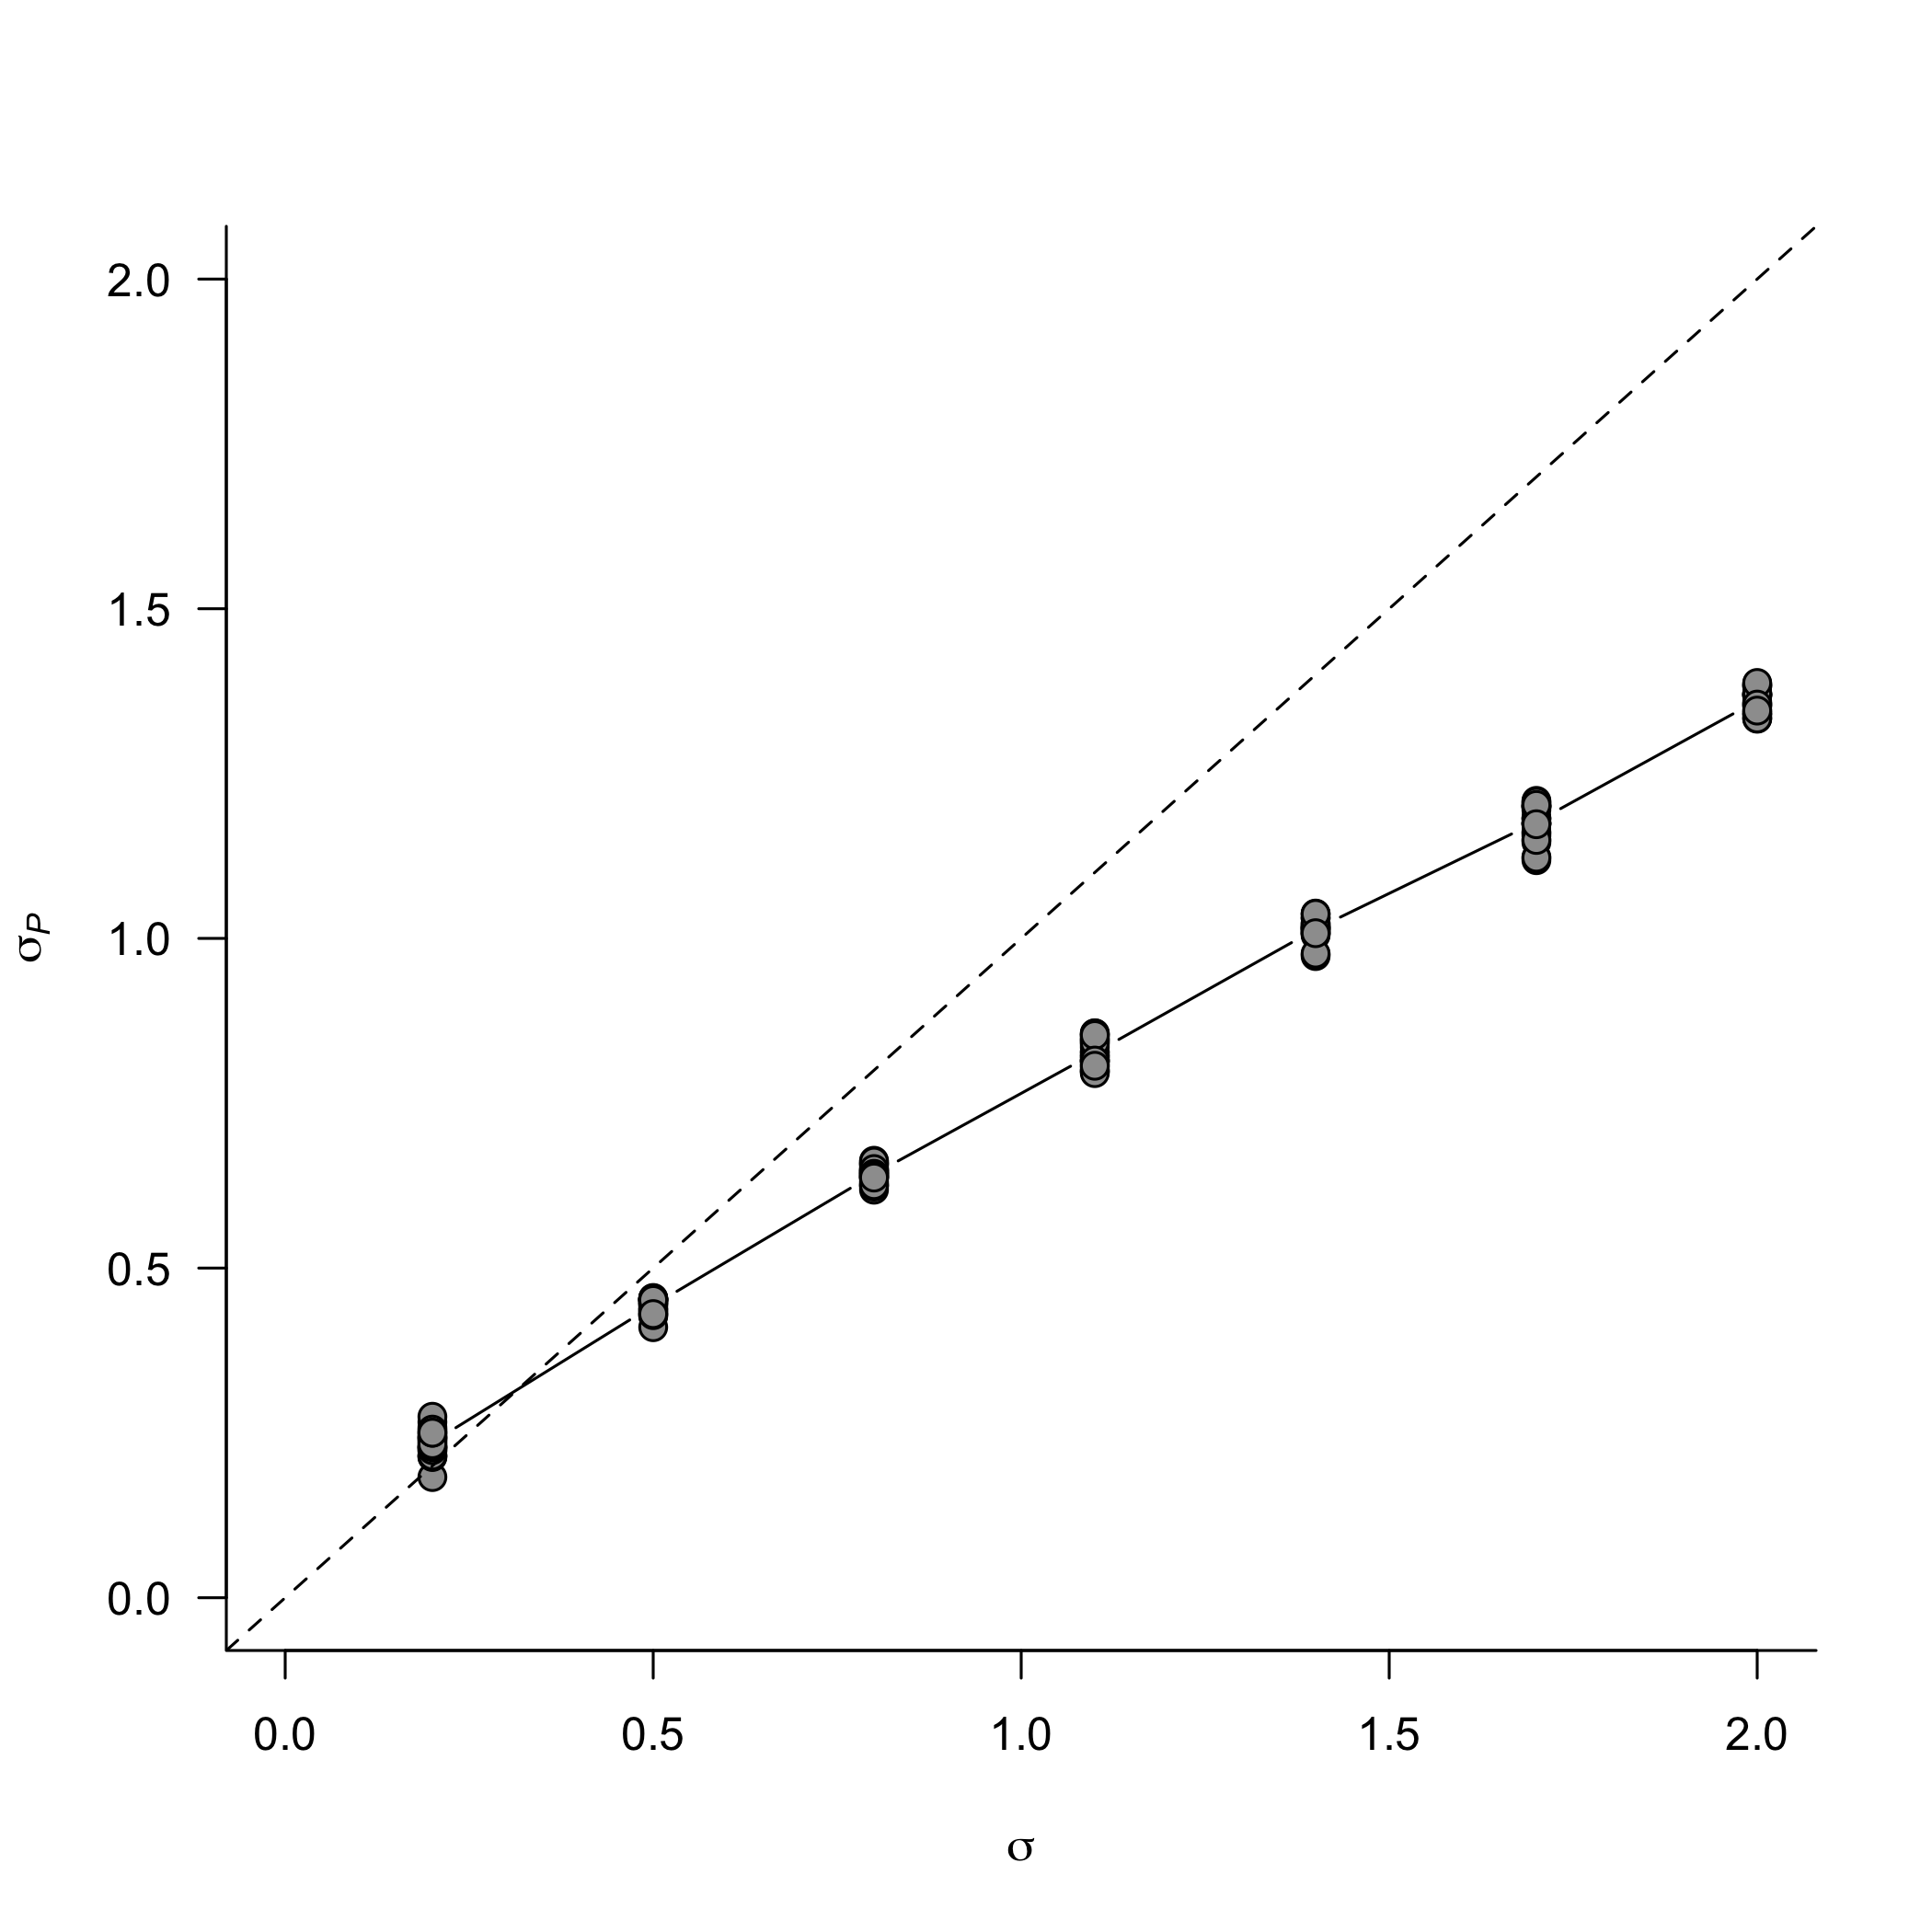
\includegraphics[width=\textwidth]{laplace-kernel-rate-estimates}
\caption{Migration rate estimates for a Laplace dispersal kernel. Each point
represents a single simulation generated under Laplace dispersal with effective
migration rate given on the x-axis and a parsimonious genome-wide estimate of
that rate on the y-axis. Estimates were conducted under three levels of 
discretization indicated by the color of the point (see main text).
The inset line shows a 1:1 relationship.
}
\label{fig:lapl-kernel-rate-estimates}
\end{figure}

\begin{figure}[h]
\centering
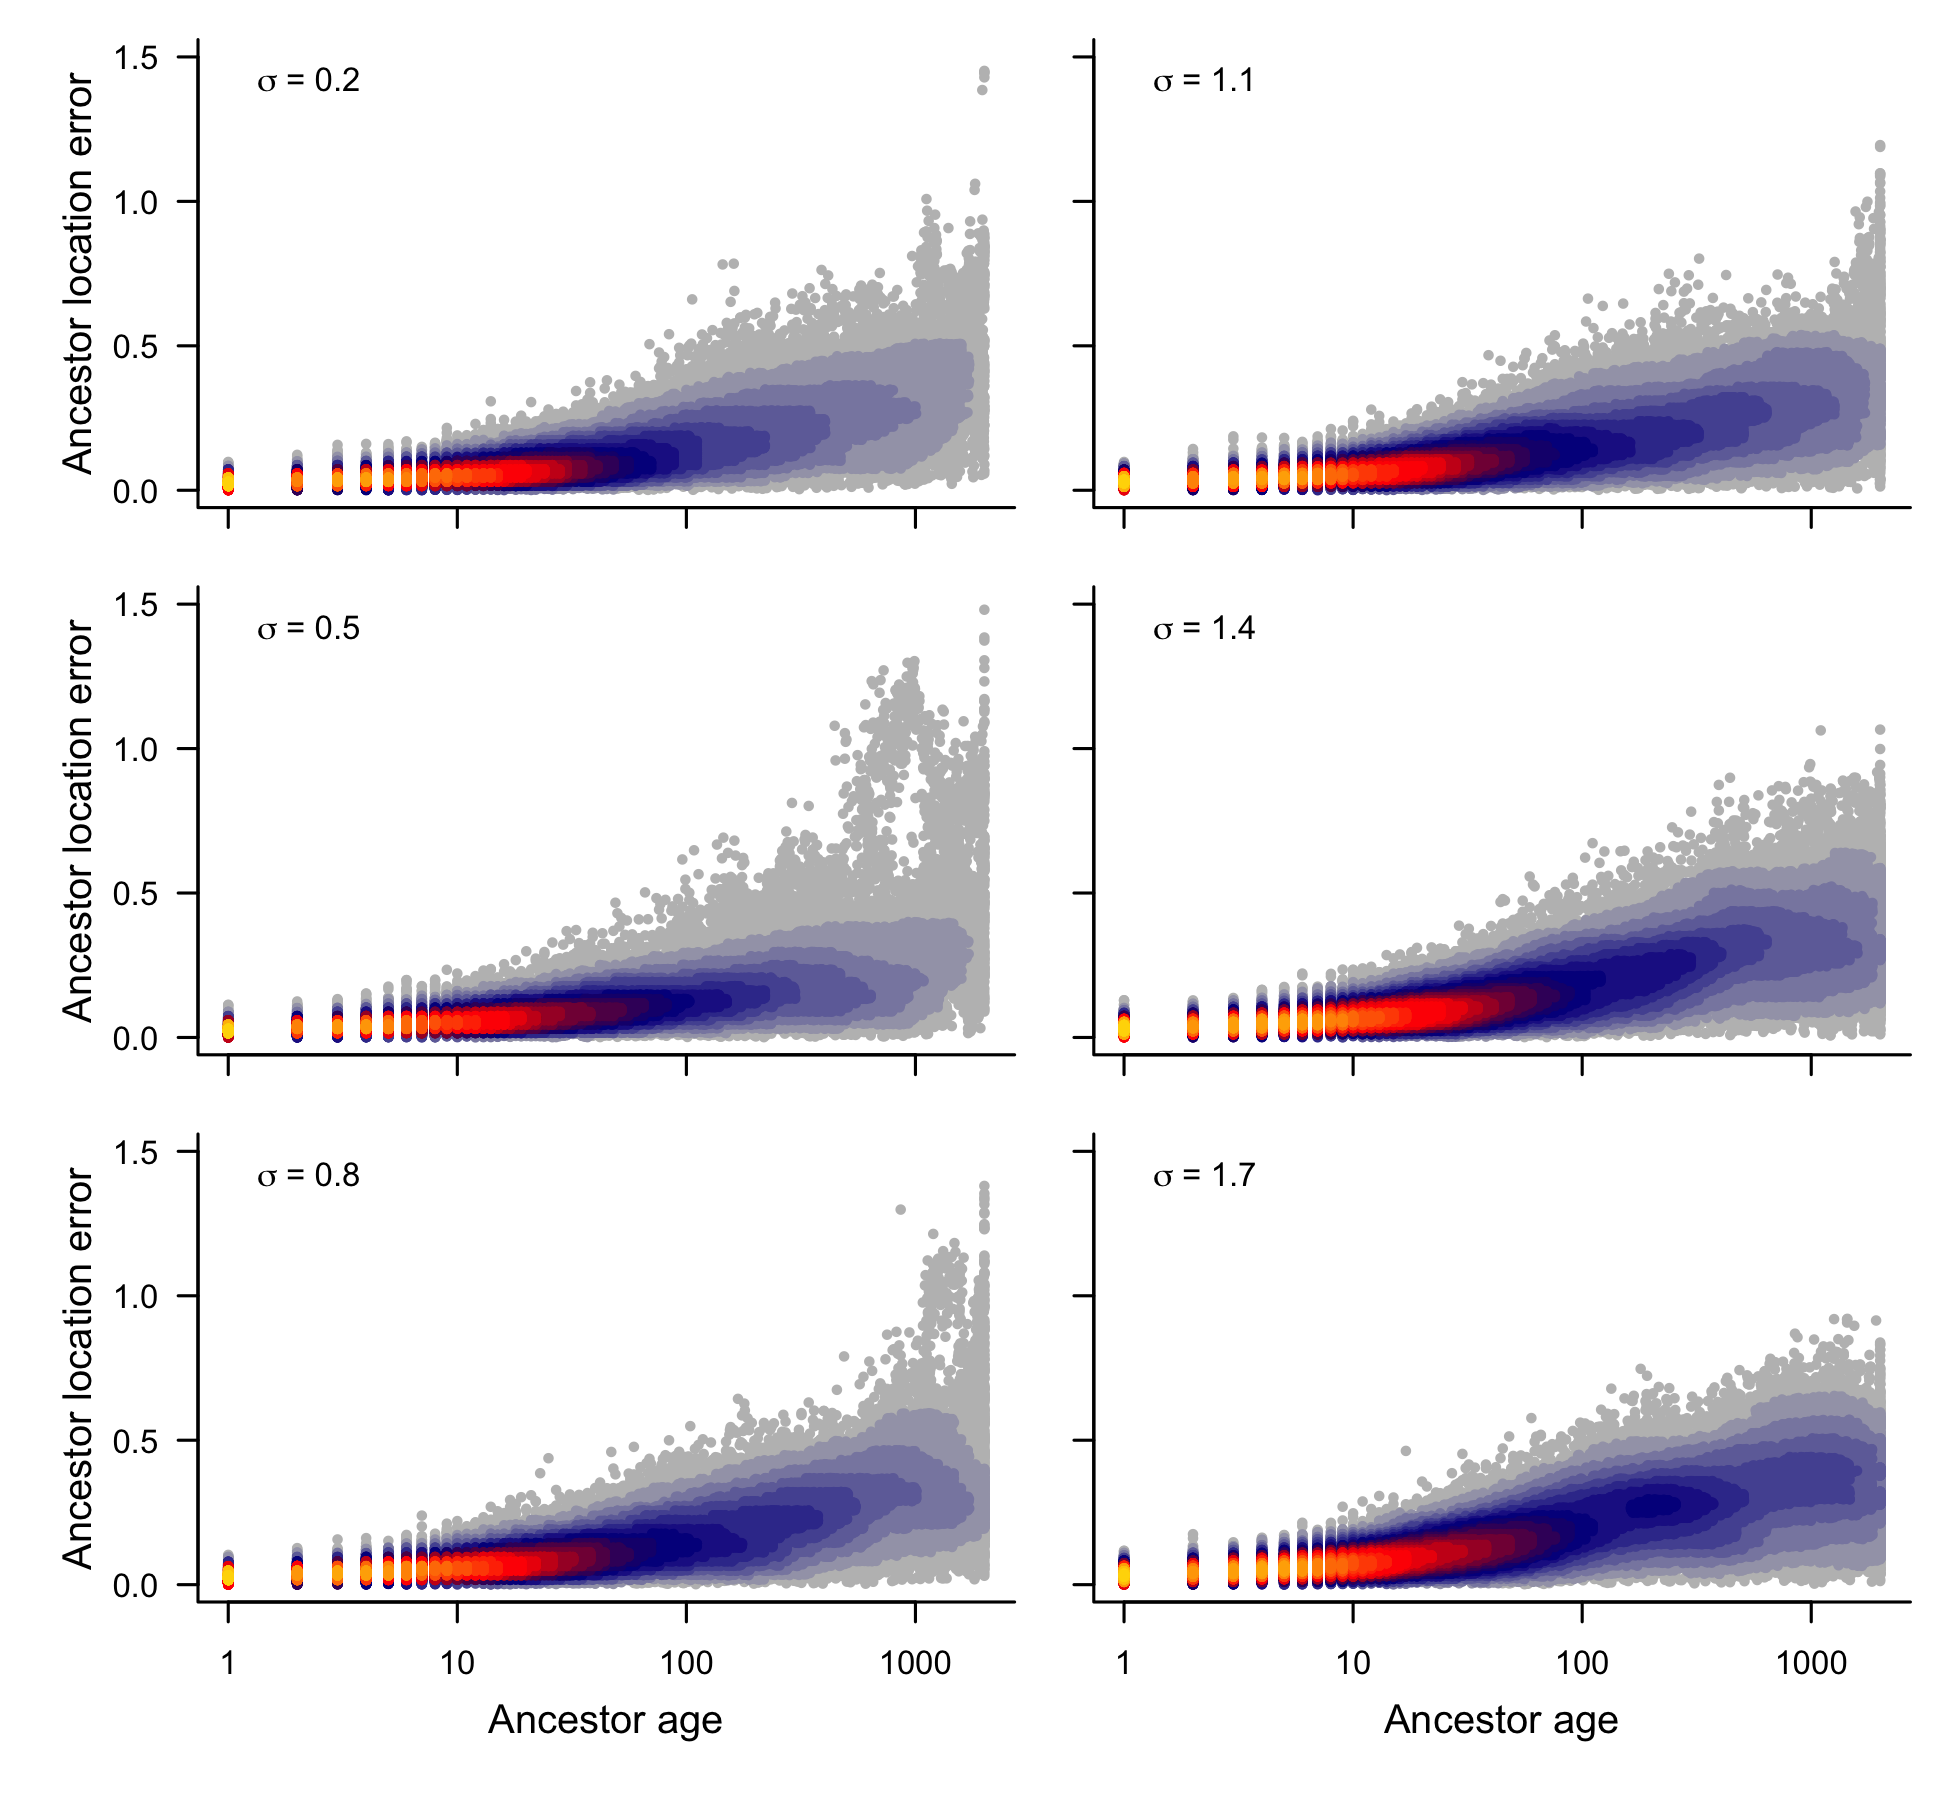
\includegraphics[width=\textwidth]{gauss-kernel-ancestor-estimates}
\caption{Ancestor location error for a Gaussian dispersal kernel. Each point
represents a single genetic ancestor. Ancestor location error is measured as
the distance between the estimated and the true location divided by the greatest
distance separating any pair of samples. Warm colors signify a greater density
of points.
}
\label{fig:gauss-kernel-ancestor-estimates}
\end{figure}

\begin{figure}[h]
\centering
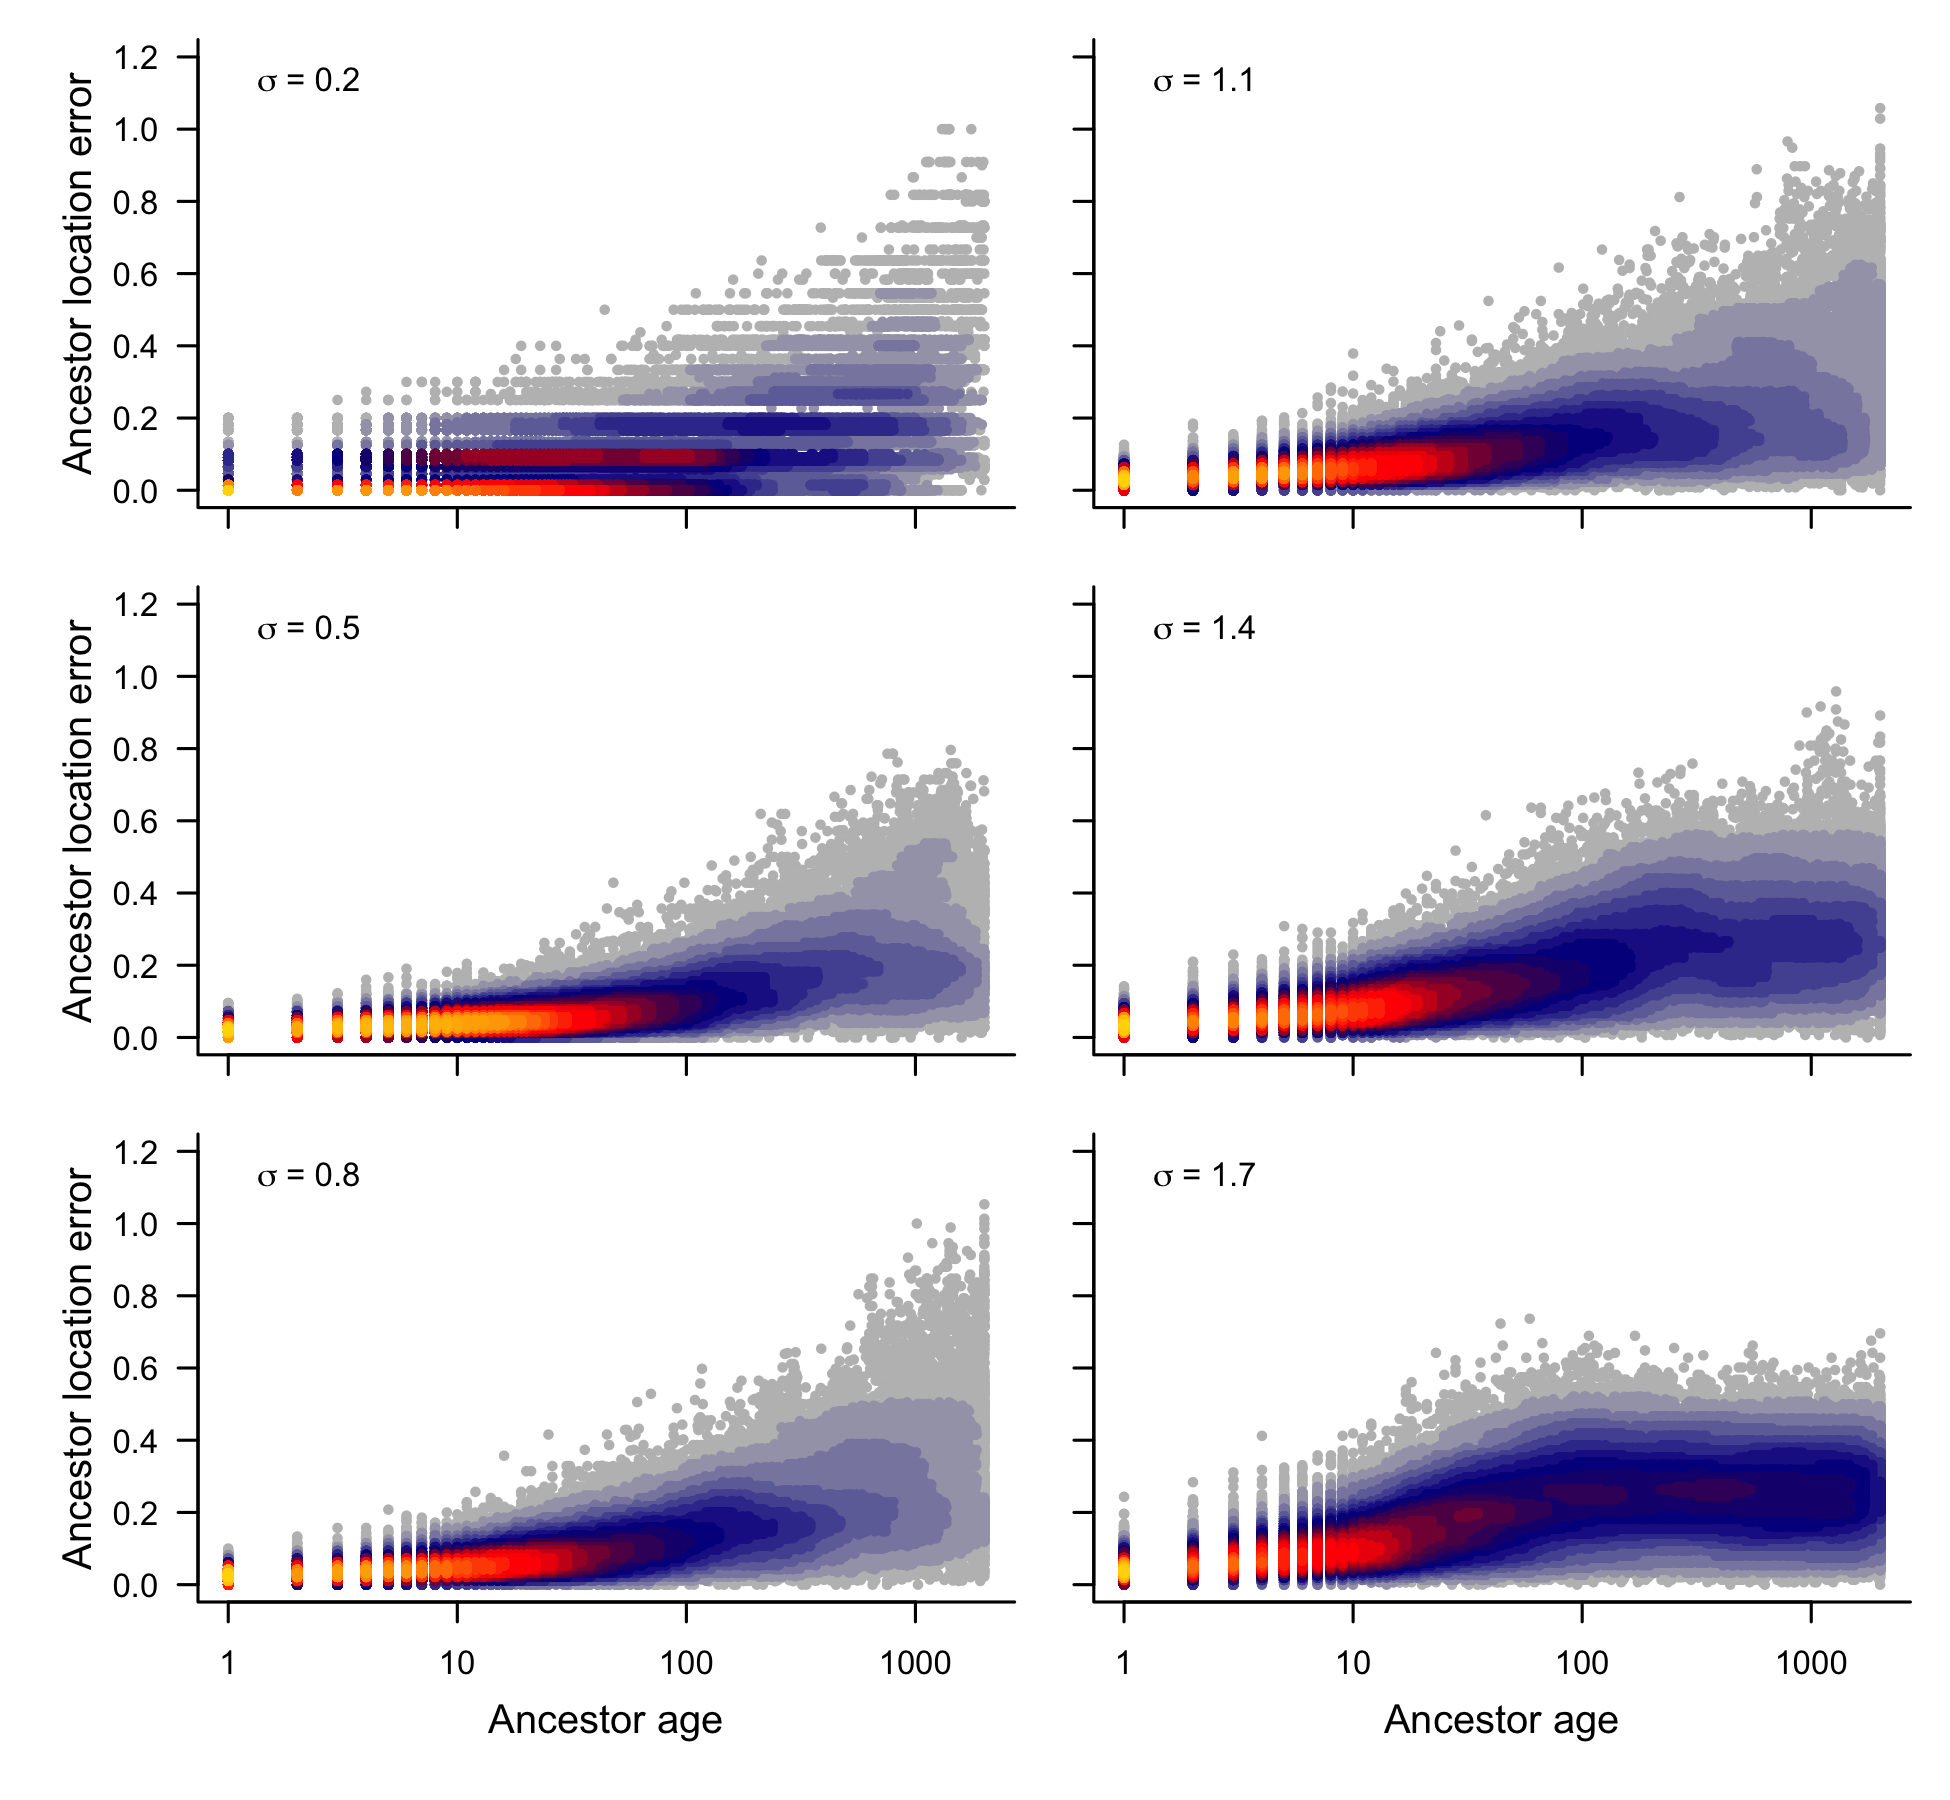
\includegraphics[width=\textwidth]{laplace-kernel-ancestor-estimates}
\caption{Ancestor location error for a Laplace dispersal kernel. Each point
represents a single genetic ancestor. Ancestor location error is measured as
the distance between the estimated and the true location divided by the greatest
distance separating any pair of samples. Warm colors signify a greater density
of points.
}
\label{fig:lapl-kernel-ancestor-estimates}
\end{figure}

\begin{figure}[h]
\centering
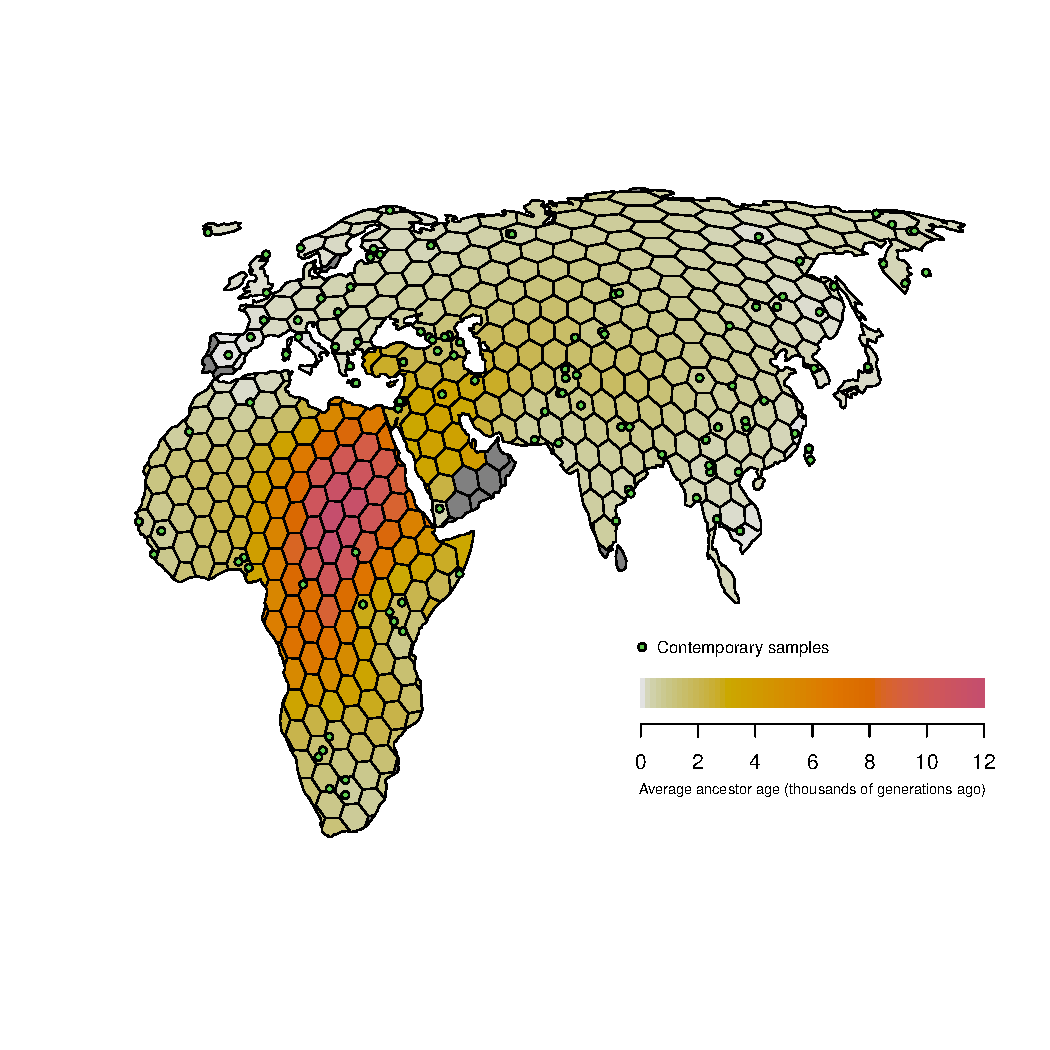
\includegraphics[width=\textwidth]{avg-ancestor-age}
\caption{Age distribution of genetic ancestors of contemporary human genome
samples. Every ancestor in the tree sequence is assigned a probability distribution 
over the set of grid cells reflecting its likely location. Each grid cell is 
colored by the weighted average of the ages of all genetic ancestors. Dark grey 
cells are omitted from the age distribution because the total weight of ancestors 
assigned to those cells is less than 1.}
\label{fig:avg-ancestor-age}
\end{figure}